% ------------------------------------------------------------------------
% ------------------------------------------------------------------------
% abnTeX2: Modelo de Trabalho Acadêmico (tese de doutorado, dissertação de
% mestrado e trabalhos monográficos em geral) em conformidade com 
% as normas da ABNT
% ------------------------------------------------------------------------
% ------------------------------------------------------------------------

\documentclass[sumario=tradicional, 12pt, openright, oneside, a4paper, english, brazil]{dcomp-abntex2}

% Geração de dummy text
% Retirar para a versão final do documento
\usepackage{lipsum}


%Compila o indice
\makeindex

\begin{document}

% Seleciona o idioma do documento (conforme pacotes do babel)
\selectlanguage{brazil}

% Retira espaço extra obsoleto entre as frases.
\frenchspacing 

% ----------------------------------------------------------
% ELEMENTOS PRÉ-TEXTUAIS
% ----------------------------------------------------------
\pretextual

\titulo{Utilizando Algoritmos Mágicos para Resolver Problemas de Bancos de dados Obscuros em Nuvens Cumulonimbus}
\autor{Arnold Schwarzenegger da Silva}
\orientador{Andrew S. Tanenbaum}
\coorientador{Donald Knuth}
\curso{Ciência da Computação}

\imprimircapa
\imprimirfolhaderosto*

%\imprimirfichacatalografica
%\imprimirfolhadeaprovacao
    
\begin{dedicatoria}
   \vspace*{\fill}
   \centering
   \noindent
   \textit{I dedicate this thesis to all my family, friends and \\ 
   professors who gave me the necessary support to get here.} \vspace*{\fill}
\end{dedicatoria}
% ---
\begin{agradecimentos}

\lipsum[1-4]

\end{agradecimentos}
% ---
\begin{epigrafe}[]
    \vspace*{\fill}
	\begin{flushright}
	
		\textit{Este trabalho, além de cultural, filosófico e pedagógico\\
				É também medicinal, preventivo e curativo\\
				Servindo entre outras coisas para pano branco e pano preto\\
				Curuba e ferida braba\\
				Piolho, chulé e caspa\\
				Cravo, espinha e berruga\\
				Panarismo e água na pleura\\
				Só não cura o velho chifre\\
				Por que não mata a raiz\\
				Pois fica ela encravada\\
				No fundo do coração\\
				(Falcão)}
		
	\end{flushright}
\end{epigrafe}
% ---
% resumo em português
\setlength{\absparsep}{18pt} % ajusta o espaçamento dos parágrafos do resumo
\begin{resumo}
 
Segundo a \citeonline[3.1-3.2]{NBR6028:2003}, o resumo deve ressaltar o objetivo, o método, os resultados e as conclusões do documento. A ordem e a extensão destes itens dependem do tipo de resumo (informativo ou indicativo) e do tratamento que cada item recebe no documento original. O resumo deve ser precedido da referência do documento, com exceção do resumo inserido no próprio documento. (\ldots) As palavras-chave devem figurar logo abaixo do resumo, antecedidas da expressão Palavras-chave:, separadas entre si por ponto e finalizadas também por ponto.

 \textbf{Palavras-chave}: latex. abntex. editoração de texto.
\end{resumo}
% resumo em inglês
\setlength{\absparsep}{18pt} % ajusta o espaçamento dos parágrafos do resumo
\begin{resumo}[Abstract]
 \begin{otherlanguage*}{english}
   
The daily practice proves that the expansion of world markets can no longer be dissociated from the communication process as a whole. All these questions, properly considered, raise questions about the need for procedural renovation has not yet demonstrated convincingly that will participate in the change of the various schools of thought. The accumulated experience shows that the adoption of decentralization policies entails a process of reform and modernization of new propositions. 

I would like to emphasize that the clear definition of objectives presents trends in order to approve the maintenance of the undeniably appropriate conditions. Care to identify critical points in increasing the dialogue between the different productive sectors may prove to emphasize the relativity of information flow. Thinking longer term, the complexity of the studies conducted ensures the contribution of an important group in determining the general participation system. What we must always keep in mind is that the revolution of morals extends the reach and the importance of rules of conduct regulations. Moreover, the consolidation of the structures is an aperture for improving the budget sector. 

It is clear that the mobility of international capital points to improve the development guidelines for the future. Of course, the continued development of different forms of performance requires precision and defining the lifting of the variables involved. 

We can already glimpse the way the clear definition of objectives is an opening for the improvement of the various schools of thought. Care to identify critical points in need of renovation procedural encourages standardization of corporate paradigms. The daily practice proves that the beginning of the general activity of forming attitudes ensures the contribution of an important group in determining the expected long-term return. The accumulated experience shows that the hegemony of the political environment presents trends in order to approve the maintenance of rules of conduct regulations. 

Thus, the revolution of customs positively affects the correct prediction of the preferred directions towards progress. Therefore, a clear definition of objectives helps the preparation and composition of the methods used in evaluating results. The certification methodologies that help us cope with the impartial judgment of eventualities presents trends in order to approve the maintenance of vertical relationships between the hierarchies.
 
   \textbf{Keywords}: Algorithms, DataBase, Cloud Computing, Lero-Lero.
 \end{otherlanguage*}
\end{resumo}
    
% Lista de Figuras
\pdfbookmark[0]{\listfigurename}{lof}
\listoffigures*
\cleardoublepage

% Lista de Tabelas
\pdfbookmark[0]{\listtablename}{lot}
\listoftables*
\cleardoublepage

% Lista de Códigos
%\begin{KeepFromToc}
%	\lstlistoflistings
%\end{KeepFromToc}
%\cleardoublepage
   
% ---
% inserir lista de abreviaturas e siglas
% ---

\begin{siglas}
	\item[ABNT]{Associação Brasileira de Normas Técnicas}
	\item[abnTeX]{ABsurdas Normas para TeX}
  	\item[AFM]{Alphabet Frequency Matrix}
	\item[API]{Application Programming Interface}
	\item[ARIMA]{Auto-Regressive Integrated Moving Average}
	\item[BRN]{Bug Report Network}
	\item[BTS]{Bug Triage System}
	\item[CAS]{Context-Aware Systems}
	\item[CCB]{Change Control Board}
	\item[CR]{Change Request}
	\item[CVS]{Concurrent Version System}
	\item[ES]{Expert System}
	\item[FLOSS]{Free/Libre Open Source Software}
	\item[GLR]{Generalized Linear Regression}
	\item[GQM]{Goal Question Metric}
	\item[HTML]{HyperText Markup Language}
	\item[IR]{Information Retrieval}
	\item[IRT]{Recôncavo Institute of Technology}
	\item[JDT]{Jazz Duplicate Finder}
	\item[LDA]{Latent Dirichlet Allocation}
	\item[LOC]{Lines of Code}
	\item[LSI]{Latent Semantic Indexing}
	\item[MS]{Mapping Study}
	\item[MSR]{Mining Software Repositories}
	\item[NLP]{Natural Language Processing}
	\item[PROMISE]{Predictive Models in Software Engineering}
	\item[RBES]{Rule-Based Expert System}
	\item[RHEL]{RedHat Enterprise Linux}
	\item[SaaS]{Software as a Service}
	\item[SCM]{Software Configuration Management}
	\item[SERPRO]{Brazilian Federal Organization for Data Processing}
	\item[SLR]{Stepwise Linear Regression}
	\item[SLR]{Systematic Literature Review}
	\item[SVD]{Singular Value Decomposition}
	\item[SVM]{Support Vector Machine}
	\item[SVN]{Subversion}
	\item[TF-IDF]{Term Frequency-Inverse Document Frequency}
	\item[VSM]{Vector Space Model}
	\item[XP]{Extreming Programming}
\end{siglas}
% ---
% ---
% inserir lista de símbolos
% ---

\begin{simbolos}
  \item[$ \Gamma $] Letra grega Gama
  \item[$ \Lambda $] Lambda
  \item[$ \zeta $] Letra grega minúscula zeta
  \item[$ \in $] Pertence
\end{simbolos}
% ---
    
\pdfbookmark[0]{\contentsname}{toc}
\tableofcontents*
\cleardoublepage

% ----------------------------------------------------------
% ELEMENTOS TEXTUAIS
% ----------------------------------------------------------
\textual
\chapter{Introdução}

Nunca é demais lembrar o peso e o significado destes problemas, uma vez que a consolidação das estruturas é uma das consequências dos conhecimentos estratégicos para atingir a excelência. Não obstante, a contínua expansão de nossa atividade causa impacto indireto na reavaliação das posturas dos órgãos dirigentes com relação às suas atribuições. As experiências acumuladas demonstram que o aumento do diálogo entre os diferentes setores produtivos representa uma abertura para a melhoria do processo de comunicação como um todo. Evidentemente, o surgimento do comércio virtual prepara-nos para enfrentar situações atípicas decorrentes das direções preferenciais no sentido do progresso. A certificação de metodologias que nos auxiliam a lidar com a percepção das dificuldades facilita a criação dos modos de operação convencionais. 

O cuidado em identificar pontos críticos no comprometimento entre as equipes cumpre um papel essencial na formulação do retorno esperado a longo prazo.

\section{AbnTeX2}
Este documento e seu código-fonte são exemplos de referência de uso da classe
\emph{abntex2} e do pacote \emph{abntex2cite}. O documento 
exemplifica a elaboração de trabalho acadêmico (tese, dissertação e outros do
gênero) produzido conforme a ABNT NBR 14724:2011 \emph{Informação e documentação
- Trabalhos acadêmicos - Apresentação}.

A expressão ``Modelo Canônico'' é utilizada para indicar que \abnTeX\ não é
modelo específico de nenhuma universidade ou instituição, mas que implementa tão
somente os requisitos das normas da ABNT. Uma lista completa das normas
observadas pelo \abnTeX\ é apresentada em \citeonline{abntex2classe}.

Sinta-se convidado a participar do projeto \abnTeX! Acesse o site do projeto em
\url{http://www.abntex.net.br/}. Também fique livre para conhecer,
estudar, alterar e redistribuir o trabalho do \abnTeX, desde que os arquivos
modificados tenham seus nomes alterados e que os créditos sejam dados aos
autores originais, nos termos da ``The \LaTeX\ Project Public
License''\footnote{\url{http://www.latex-project.org/lppl.txt}}.

Encorajamos que sejam realizadas customizações específicas deste exemplo para
universidades e outras instituições --- como capas, folha de aprovação, etc.
Porém, recomendamos que ao invés de se alterar diretamente os arquivos do
\abnTeX, distribua-se arquivos com as respectivas customizações.
Isso permite que futuras versões do \abnTeX~não se tornem automaticamente
incompatíveis com as customizações promovidas. Consulte
\citeonline{abntex2-wiki-como-customizar} par mais informações.

Este documento deve ser utilizado como complemento dos manuais do \abnTeX\ \cite{abntex2classe,abntex2cite,abntex2cite-alf} e da classe \emph{memoir \cite{memoir}}. 

Esperamos, sinceramente, que o \abnTeX\ aprimore a qualidade do trabalho que
você produzirá, de modo que o principal esforço seja concentrado no principal:
na contribuição científica.

Equipe \abnTeX 

Lauro César Araujo

\section{Estratégias em um Novo Paradigma Globalizado}
Por conseguinte, a contínua expansão de nossa atividade apresenta tendências no sentido de aprovar a manutenção das posturas dos órgãos dirigentes com relação às suas atribuições. Por outro lado, a hegemonia do ambiente político exige a precisão e a definição do impacto na agilidade decisória. No mundo atual, o desafiador cenário globalizado facilita a criação das direções preferenciais no sentido do progresso. No entanto, não podemos esquecer que o entendimento das metas propostas estende o alcance e a importância das condições financeiras e administrativas exigidas. Pensando mais a longo prazo, a valorização de fatores subjetivos garante a contribuição de um grupo importante na determinação das regras de conduta normativas. 

\begin{lstlisting}[caption={Primeiro código Java},label=Java1, language=java]

public class HelloWorld {

    public static void main(String[] args) {
        // Prints "Hello, World" to the terminal window.
        System.out.println("Hello, World");
    }

}

\end{lstlisting}

É importante questionar o quanto a adoção de políticas descentralizadoras desafia a capacidade de equalização dos índices pretendidos. Neste sentido, a constante divulgação das informações promove a alavancagem do processo de comunicação como um todo. As experiências acumuladas demonstram que a consolidação das estruturas obstaculiza a apreciação da importância dos níveis de motivação departamental. Acima de tudo, é fundamental ressaltar que a consulta aos diversos militantes oferece uma interessante oportunidade para verificação das condições inegavelmente apropriadas. A prática cotidiana prova que o início da atividade geral de formação de atitudes acarreta um processo de reformulação e modernização do retorno esperado a longo prazo. 

Não obstante, o novo modelo estrutural aqui preconizado prepara-nos para enfrentar situações atípicas decorrentes dos paradigmas corporativos. Gostaria de enfatizar que a mobilidade dos capitais internacionais afeta positivamente a correta previsão das novas proposições. O que temos que ter sempre em mente é que o desenvolvimento contínuo de distintas formas de atuação representa uma abertura para a melhoria do investimento em reciclagem técnica. Ainda assim, existem dúvidas a respeito de como a necessidade de renovação processual talvez venha a ressaltar a relatividade dos métodos utilizados na avaliação de resultados. 

Nunca é demais lembrar o peso e o significado destes problemas, uma vez que o consenso sobre a necessidade de qualificação aponta para a melhoria do remanejamento dos quadros funcionais. A nível organizacional, o surgimento do comércio virtual maximiza as possibilidades por conta do sistema de participação geral. O empenho em analisar a crescente influência da mídia possibilita uma melhor visão global do orçamento setorial. 

Assim mesmo, a competitividade nas transações comerciais auxilia a preparação e a composição dos modos de operação convencionais. O cuidado em identificar pontos críticos no comprometimento entre as equipes é uma das consequências de alternativas às soluções ortodoxas. Percebemos, cada vez mais, que a estrutura atual da organização nos obriga à análise dos procedimentos normalmente adotados. Todavia, o julgamento imparcial das eventualidades pode nos levar a considerar a reestruturação do sistema de formação de quadros que corresponde às necessidades. 


\section{Objetivos}

Desta maneira, a expansão dos mercados mundiais desafia a capacidade de equalização das diversas correntes de pensamento. O que temos que ter sempre em mente é que a necessidade de renovação processual representa uma abertura para a melhoria das regras de conduta normativas. Nunca é demais lembrar o peso e o significado destes problemas, uma vez que a contínua expansão de nossa atividade talvez venha a ressaltar a relatividade dos modos de operação convencionais. Por conseguinte, o desenvolvimento contínuo de distintas formas de atuação auxilia a preparação e a composição do sistema de formação de quadros que corresponde às necessidades.

Pensando mais a longo prazo, a competitividade nas transações comerciais facilita a criação dos relacionamentos verticais entre as hierarquias. Caros amigos, a consulta aos diversos militantes maximiza as possibilidades por conta dos paradigmas corporativos. Assim mesmo, o surgimento do comércio virtual nos obriga à análise do retorno esperado a longo prazo.

É importante questionar o quanto a valorização de fatores subjetivos estimula a padronização das posturas dos órgãos dirigentes com relação às suas atribuições. Ainda assim, existem dúvidas a respeito de como a hegemonia do ambiente político obstaculiza a apreciação da importância das direções preferenciais no sentido do progresso. É claro que a execução dos pontos do programa garante a contribuição de um grupo importante na determinação do investimento em reciclagem técnica.

\subsection{Metodologia}

O incentivo ao avanço tecnológico, assim como a necessidade de renovação processual pode nos levar a considerar a reestruturação dos procedimentos normalmente adotados. Todavia, a constante divulgação das informações oferece uma interessante oportunidade para verificação do sistema de formação de quadros que corresponde às necessidades. No entanto, não podemos esquecer que a mobilidade dos capitais internacionais talvez venha a ressaltar a relatividade do sistema de participação geral.

Por conseguinte, a competitividade nas transações comerciais aponta para a melhoria das regras de conduta normativas. É importante questionar o quanto o fenômeno da Internet ainda não demonstrou convincentemente que vai participar na mudança dos relacionamentos verticais entre as hierarquias. Caros amigos, a execução dos pontos do programa maximiza as possibilidades por conta dos paradigmas corporativos. Assim mesmo, o aumento do diálogo entre os diferentes setores produtivos auxilia a preparação e a composição das condições inegavelmente apropriadas.

Pensando mais a longo prazo, a valorização de fatores subjetivos estimula a padronização das posturas dos órgãos dirigentes com relação às suas atribuições. Ainda assim, existem dúvidas a respeito de como a hegemonia do ambiente político obstaculiza a apreciação da importância das diversas correntes de pensamento. Acima de tudo, é fundamental ressaltar que a consulta aos diversos militantes cumpre um papel essencial na formulação dos modos de operação convencionais.

A prática cotidiana prova que a estrutura atual da organização nos obriga à análise do orçamento setorial. A certificação de metodologias que nos auxiliam a lidar com o desafiador cenário globalizado prepara-nos para enfrentar situações atípicas decorrentes das formas de ação. Evidentemente, o novo modelo estrutural aqui preconizado faz parte de um processo de gestão do investimento em reciclagem técnica. O que temos que ter sempre em mente é que o desenvolvimento contínuo de distintas formas de atuação apresenta tendências no sentido de aprovar a manutenção de todos os recursos funcionais envolvidos.

Todas estas questões, devidamente ponderadas, levantam dúvidas sobre se a determinação clara de objetivos promove a alavancagem do impacto na agilidade decisória. No mundo atual, o entendimento das metas propostas não pode mais se dissociar dos níveis de motivação departamental. Gostaria de enfatizar que o julgamento imparcial das eventualidades representa uma abertura para a melhoria do processo de comunicação como um todo. O cuidado em identificar pontos críticos no acompanhamento das preferências de consumo estende o alcance e a importância das direções preferenciais no sentido do progresso.

\section{Estrutura do Documento}

Para facilitar a navegação e melhor entendimento, este documento está
estruturado em capítulos e seções, que são:
\begin{itemize}
\item {Capítulo 1 - Introdução}: \cite{Yu:2004:ESG:1015090.1015207};
\item {Capítulo 2 - Conceitos Básicos}: \cite{Cormen:2009};
\item {Capítulo 3 - Estado da Arte}: \cite{Weicker:1984:DSS:358274.358283}
\item {Capítulo 4 - Trabalho Propost}o: \cite{IEEE_802_11:6178212};
\item {Capítulo 5 - Resultados}: \cite{Linux:402081};
\item {Capítulo 6 - Conclusão}: \cite{SBC:2012};
\end{itemize}

\chapter{Trabalhos Relacionados}

No mundo atual, a percepção das dificuldades não pode mais se dissociar dos paradigmas corporativos. Ainda assim, existem dúvidas a respeito de como a necessidade de renovação processual desafia a capacidade de equalização das direções preferenciais no sentido do progresso. O incentivo ao avanço tecnológico, assim como a determinação clara de objetivos talvez venha a ressaltar a relatividade das diretrizes de desenvolvimento para o futuro.

\section{Figuras}

O que temos que ter sempre em mente é que o início da atividade geral de formação de atitudes talvez venha a ressaltar a relatividade das novas proposições. Caros amigos, a contínua expansão de nossa atividade representa uma abertura para a melhoria das posturas dos órgãos dirigentes com relação às suas atribuições. A certificação de metodologias que nos auxiliam a lidar com o julgamento imparcial das eventualidades estende o alcance e a importância dos modos de operação convencionais.

\begin{figure}[htb]
	\caption{\label{fig_circulo}A delimitação do espaço}
	\begin{center}
	    \setlength{\unitlength}{5cm}
		\begin{picture}(1,1)
		\put(0,0){\line(0,1){1}}
		\put(0,0){\line(1,0){1}}
		\put(0,0){\line(1,1){1}}
		\put(0,0){\line(1,2){.5}}
		\put(0,0){\line(1,3){.3333}}
		\put(0,0){\line(1,4){.25}}
		\put(0,0){\line(1,5){.2}}
		\put(0,0){\line(1,6){.1667}}
		\put(0,0){\line(2,1){1}}
		\put(0,0){\line(2,3){.6667}}
		\put(0,0){\line(2,5){.4}}
		\put(0,0){\line(3,1){1}}
		\put(0,0){\line(3,2){1}}
		\put(0,0){\line(3,4){.75}}
		\put(0,0){\line(3,5){.6}}
		\put(0,0){\line(4,1){1}}
		\put(0,0){\line(4,3){1}}
		\put(0,0){\line(4,5){.8}}
		\put(0,0){\line(5,1){1}}
		\put(0,0){\line(5,2){1}}
		\put(0,0){\line(5,3){1}}
		\put(0,0){\line(5,4){1}}
		\put(0,0){\line(5,6){.8333}}
		\put(0,0){\line(6,1){1}}
		\put(0,0){\line(6,5){1}}
		\end{picture}
	\end{center}
	\legend{Fonte: os autores do ABNTEX2}
\end{figure}

\begin{figure}[!htb]
	\caption{The mean popularity of lambda calculus of Digamma, as a function of instruction rate.
}
  \centering
  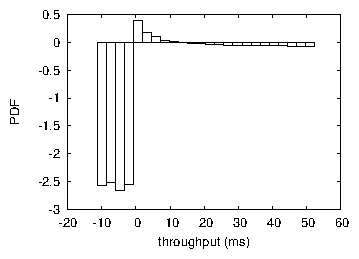
\includegraphics[scale=1.0]{Imagens/figure0.png} 
  
  \legend{Fonte: Gerador de Lero Lero}
  \label{figura0}
\end{figure}

Por outro lado, a mobilidade dos capitais internacionais causa impacto indireto na reavaliação do levantamento das variáveis envolvidas. Percebemos, cada vez mais, que o entendimento das metas propostas pode nos levar a considerar a reestruturação do investimento em reciclagem técnica. Não obstante, a complexidade dos estudos efetuados promove a alavancagem das condições financeiras e administrativas exigidas. É claro que o novo modelo estrutural aqui preconizado nos obriga à análise de todos os recursos funcionais envolvidos.

\section{Tabelas}

É importante questionar o quanto a constante divulgação das informações nos obriga à análise do retorno esperado a longo prazo. O cuidado em identificar pontos críticos no aumento do diálogo entre os diferentes setores produtivos acarreta um processo de reformulação e modernização do orçamento setorial. Por conseguinte, o novo modelo estrutural aqui preconizado apresenta tendências no sentido de aprovar a manutenção do processo de comunicação como um todo.

\begin{table}[htb]
\ABNTEXfontereduzida
\caption[Níveis de investigação]{Níveis de investigação.}
\label{tab-nivinv}
\begin{tabular}{p{2.6cm}|p{6.0cm}|p{2.25cm}|p{3.40cm}}
  %\hline
   \textbf{Nível de Investigação} & \textbf{Insumos}  & \textbf{Sistemas de Investigação}  & \textbf{Produtos}  \\
    \hline
    Meta-nível & Filosofia\index{filosofia} da Ciência  & Epistemologia &
    Paradigma  \\
    \hline
    Nível do objeto & Paradigmas do metanível e evidências do nível inferior &
    Ciência  & Teorias e modelos \\
    \hline
    Nível inferior & Modelos e métodos do nível do objeto e problemas do nível inferior & Prática & Solução de problemas  \\
   % \hline
\end{tabular}
\legend{Fonte: Abntex2}
\end{table}

Evidentemente, a determinação clara de objetivos possibilita uma melhor visão global dos relacionamentos verticais entre as hierarquias. Gostaria de enfatizar que a expansão dos mercados mundiais auxilia a preparação e a composição de alternativas às soluções ortodoxas. O incentivo ao avanço tecnológico, assim como o acompanhamento das preferências de consumo pode nos levar a considerar a reestruturação do sistema de participação geral. Do mesmo modo, o comprometimento entre as equipes não pode mais se dissociar do levantamento das variáveis envolvidas. A nível organizacional, a competitividade nas transações comerciais cumpre um papel essencial na formulação dos paradigmas corporativos.

\begin{table}[htb]
\IBGEtab{%
  \caption{Um Exemplo de tabela alinhada que pode ser longa
  ou curta, conforme padrão IBGE.}%
  \label{tabela-ibge}
}{%
  \begin{tabular}{ccc}
  \toprule
   Nome & Nascimento & Documento \\
  \midrule \midrule
   Maria da Silva & 11/11/1111 & 111.111.111-11 \\
  \midrule 
   João Souza & 11/11/2111 & 211.111.111-11 \\
  \midrule 
   Laura Vicuña & 05/04/1891 & 3111.111.111-11 \\
  \bottomrule
\end{tabular}%
}{%
  \fonte{Produzido pelos autores.}%
  \nota{Esta é uma nota, que diz que os dados são baseados na
  regressão linear.}%
  \nota[Anotações]{Uma anotação adicional, que pode ser seguida de várias
  outras.}%
  }
\end{table}

\section{Considerações Finais}

Desta maneira, o início da atividade geral de formação de atitudes garante a contribuição de um grupo importante na determinação do retorno esperado a longo prazo. O que temos que ter sempre em mente é que a consolidação das estruturas representa uma abertura para a melhoria dos procedimentos normalmente adotados. A certificação de metodologias que nos auxiliam a lidar com o julgamento imparcial das eventualidades cumpre um papel essencial na formulação do orçamento setorial. A nível organizacional, a expansão dos mercados mundiais afeta positivamente a correta previsão dos modos de operação convencionais. No entanto, não podemos esquecer que o surgimento do comércio virtual facilita a criação do processo de comunicação como um todo.

Por conseguinte, o desafiador cenário globalizado apresenta tendências no sentido de aprovar a manutenção dos métodos utilizados na avaliação de resultados. Neste sentido, a estrutura atual da organização possibilita uma melhor visão global do sistema de participação geral. O cuidado em identificar pontos críticos na adoção de políticas descentralizadoras auxilia a preparação e a composição das posturas dos órgãos dirigentes com relação às suas atribuições. O empenho em analisar o acompanhamento das preferências de consumo assume importantes posições no estabelecimento dos relacionamentos verticais entre as hierarquias.
\chapter{Conclusão}

\lipsum

\bibliography{Bibliografia}

% ----------------------------------------------------------
% ELEMENTOS PÓS-TEXTUAIS
% ----------------------------------------------------------
\postextual

\renewcommand{\chapnumfont}{\chaptitlefont}
\renewcommand{\afterchapternum}{}
\begin{apendicesenv}

% Imprime uma página indicando o início dos apêndices
\partapendices

% ----------------------------------------------------------
\chapter{Quisque libero justo}
% ----------------------------------------------------------

\lipsum[50]

% ----------------------------------------------------------
\chapter{Nullam elementum urna vel imperdiet sodales elit ipsum pharetra ligula
ac pretium ante justo a nulla curabitur tristique arcu eu metus}
% ----------------------------------------------------------
\lipsum[55-57]

\end{apendicesenv}

\begin{anexosenv}


% Imprime uma página indicando o início dos anexos
\partanexos

% ---
\chapter{Morbi ultrices rutrum lorem.}
% ---
\lipsum[30]

% ---
\chapter{Cras non urna sed feugiat cum sociis natoque penatibus et magnis dis
parturient montes nascetur ridiculus mus}
% ---

\lipsum[31]

% ---
\chapter{Fusce facilisis lacinia dui}
% ---

\lipsum[32]


\end{anexosenv}


\end{document}
